\section{Thu, Sep 6, 2018}

\subsection{7:30 AM}

Found an interesting thing today. Not sure if I've ever figured this one out or not
before?

The below will not compile.

\lstinputlisting[language=Java]{2018/TestCase.java}

It throws the following error:

\begin{displayquote}
TestCase.java:14: error: variable found is already defined in method main(String[])
        boolean found = true;
\end{displayquote}

So variables within case statements carry onward thorugh the switch. Interesting
indeed.

\subsection{9:00 AM}

This month in 1993, six members of the LDS church were either excommunicated or
disfellowshipped. It ranges on a couple of different topics of why they were
disciplined by the church. I find it interesting that one was disciplined for
teaching of a Mother in Heaven, when there is a hymn that clearly states there's
probably a Mother in Heaven. I will have to read further on what they wrote to see
what was so controversial about the topic.

Others were exed because they spoke the truth. Speaking the truth about the church's
history is apparently not a good thing. I do not know why that would be, I mean is it
not the truth we seek after? No matter what it is?

I started studying church history in May of this year. Been studying it since that
time. I don't see a point where I will stop studying it yet, there is so much to go
over and so much to discover about it all. It really is fascinating.

The other day I wrote about the three degrees of glory not beig found in the Book of
Mormon. Other teachings not found in the book are baptism for the dead and polygamy.
Other than polygamy being wrong and that the Nephites shouldn't take more than one
wife. For a book that's supposed to contain precious parts of the Bible that was
lost, it does appear to be missing some things and lacking.

There is the sealed portion of the plates which we do not have. That was to come at a
much later date, but the church is under condemnation because it has forgotten the
Book of Mormon. So until that condemnation is removed, the saints will not be able to
enjoy the sealed portion.

President Ezra Taft Bension said:

\begin{displayquote}
``Unless we read the Book of Mormon and give heed to its teachings, the Lord has stated 
in section 84 of the Doctrine and Covenants that the whole Church is under 
condemnation" and ``In our day, the Lord has revealed the need to reemphasize the 
Book of Mormon to get the Church and all the children of Zion out from under 
condemnation—the scourge and judgment."\footnote{Ensign, May 1986, pp. 5, 78.}
\end{displayquote}

Here's the verses from the Doctrine and Covenants:

\begin{displayquote}
And your minds in times past have been darkened because of unbelief, and because you 
have treated lightly the things you have received-

Which vanity and unbelief have brought the whole church under condemnation.

And this condemnation resteth upon the children of Zion, even all.

And they shall remain under this condemnation until they repent and remember the new 
covenant, even the Book of Mormon and the former commandments which I have given 
them, not only to say, but to do according to that which I have written.\footnote{
D\&C 84:54-57
}
\end{displayquote}

It goes back to the thought, if you don't appreciate what you have now, why would you
expect more? It's an interesting thought to be sure. But even if the saints back then
weren't remembering the Book of Mormon and it's been how long? That's quite a bit of
time for a membership to not follow the teachings of its leaders.\footnote{Section 84
was given in Ohio on September 22 and 23, 1832.} 

\subsection{2:27 PM}

In a talk titled ``The Mantle Is Far, Far Greater Than the Intellect"\footnote{
https://www.lds.org/manual/teaching-seminary-preservice-readings-religion-370-471-and-475/the-mantle-is-far-far-greater-than-the-intellect?lang=eng
}, Boyd K. Packer
said the following:

\begin{figure}[h!]
  \centering
  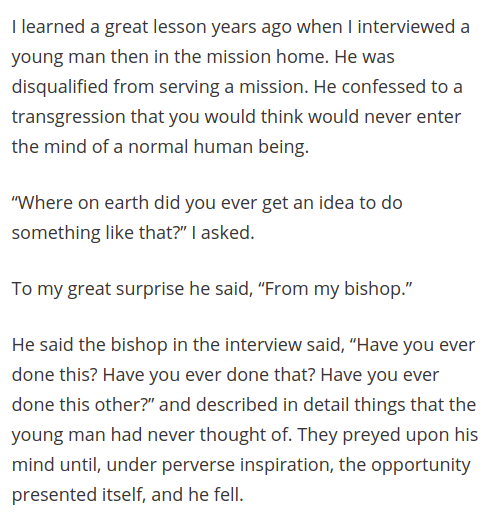
\includegraphics[width=1\linewidth]{2018/images/bishop.png}
  \caption{From my bishop}
  \label{fig:clayton3}
\end{figure}

I have no words for this. Such thoughts should not be placed in the minds of
impressionable youth. This talk was originally given in 1981. It's currently on the
church's website. Yet, they don't follow this simple rule to this day. Some bishops
do, not all though. Having one bishop do this is unthinkable and wrong. One is too
many.